\documentclass[aspectratio=169]{beamer} 
\usepackage[T1]{fontenc}
\usepackage[utf8]{inputenc}
\usepackage{plex-sans}
\usepackage[scale=0.85]{plex-mono}
\usepackage{amsmath}
\usepackage{amssymb}
\usepackage[british]{babel}
\usepackage[backend=biber,style=alphabetic-verb,citetracker=true]{biblatex}
\usepackage{csquotes}
\usepackage{hyperref}
\usepackage[overlay, absolute]{textpos}
\usepackage{tikz}
\usepackage{graphicx}
\usepackage{booktabs}
\usepackage{subcaption}
\usepackage{transparent}
\usepackage{multicol}

% TikZ libraries for relative positioning and better looking arrows
\usetikzlibrary{positioning, arrows.meta}

% BibLaTeX sources
\addbibresource{literature.bib}

% Urls the same color as text
\urlstyle{same}

% Use numbers instead of icons in the bibliography
\setbeamertemplate{bibliography item}[text]

% B&W color theme
\usecolortheme{seagull}

% Use symbols instead of numbers for footnotes
\renewcommand{\thefootnote}{\fnsymbol{footnote}}

% don't show Beamer buttons
\beamertemplatenavigationsymbolsempty

% more spacing below footnotes
\setbeamertemplate{footline}{\vspace{6.7pt}} 

%Information to be included in the title page:
\title{Tools for Gossip} 
\subtitle{Bachelor's Project} 
\author{%
    R.A. Meffert\\\vspace{5pt}
    {\small Supervisor: Dr. B.R.M Gattinger} 
} 
\institute{University of Groningen} 
\date{Bachelor's Symposium, January 25, 2021}

\begin{document}
{\setbeamertemplate{background}
{\transparent{0.2}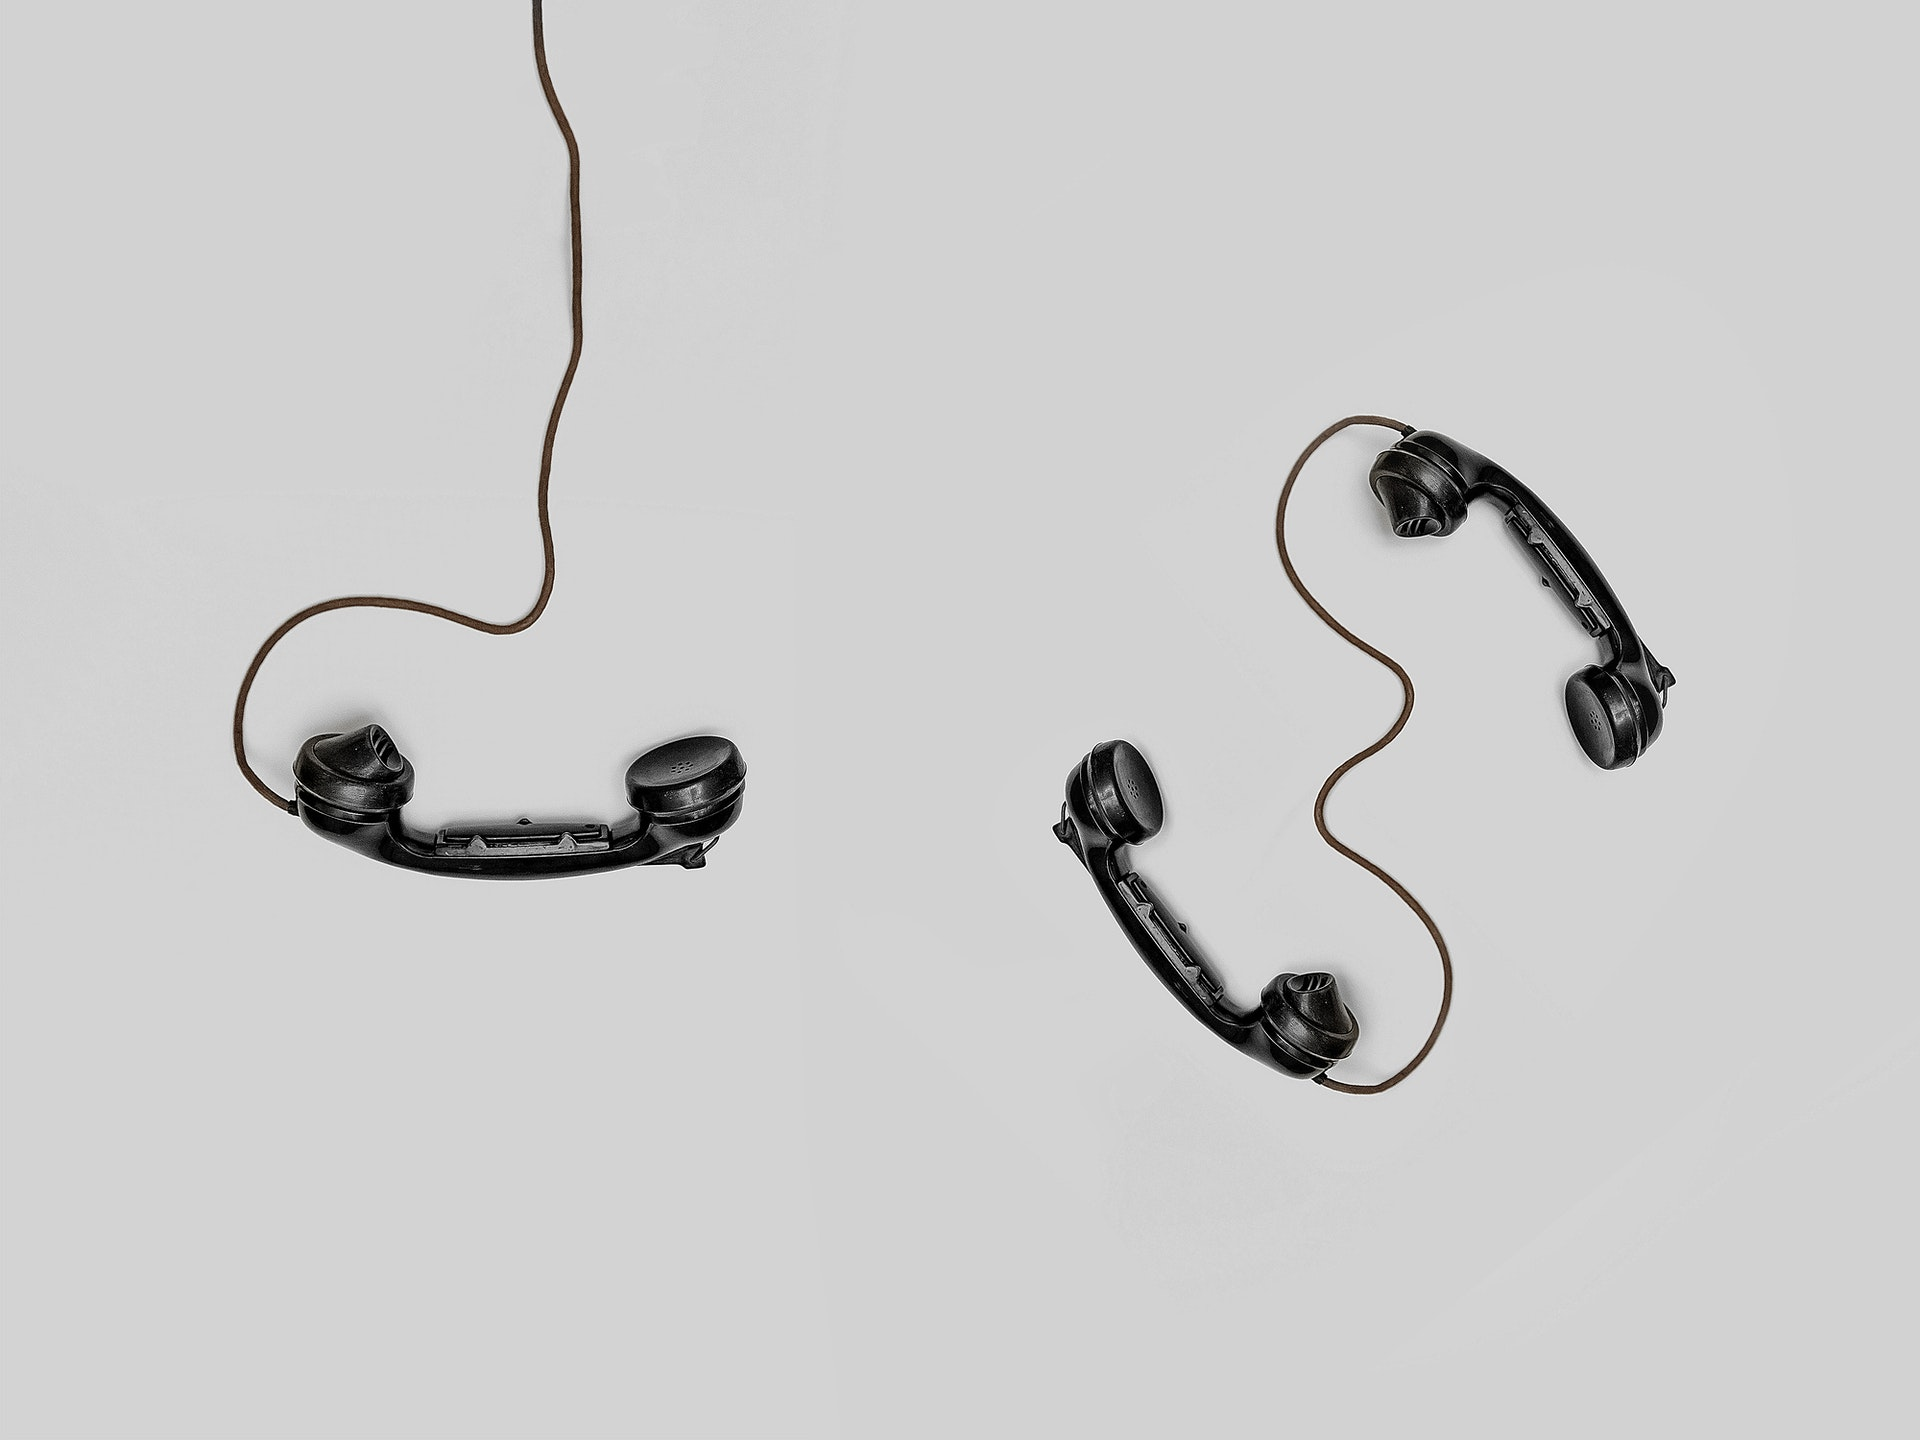
\includegraphics[width=\paperwidth,keepaspectratio]{phone.jpg}}
\frame{\titlepage}
}
\begin{frame}[c]{About this bachelor's project}
    \begin{multicols}{2}
        \begin{itemize}
            \item<1-> The telephone problem \parencite[e.g.][]{tijdeman_telephone_1971}
            \item<2-> Dynamic gossip \cite{van_ditmarsch_dynamic_2018}
            \item<3-> Goal: intuitive, educational tool
        \end{itemize}
        \columnbreak
        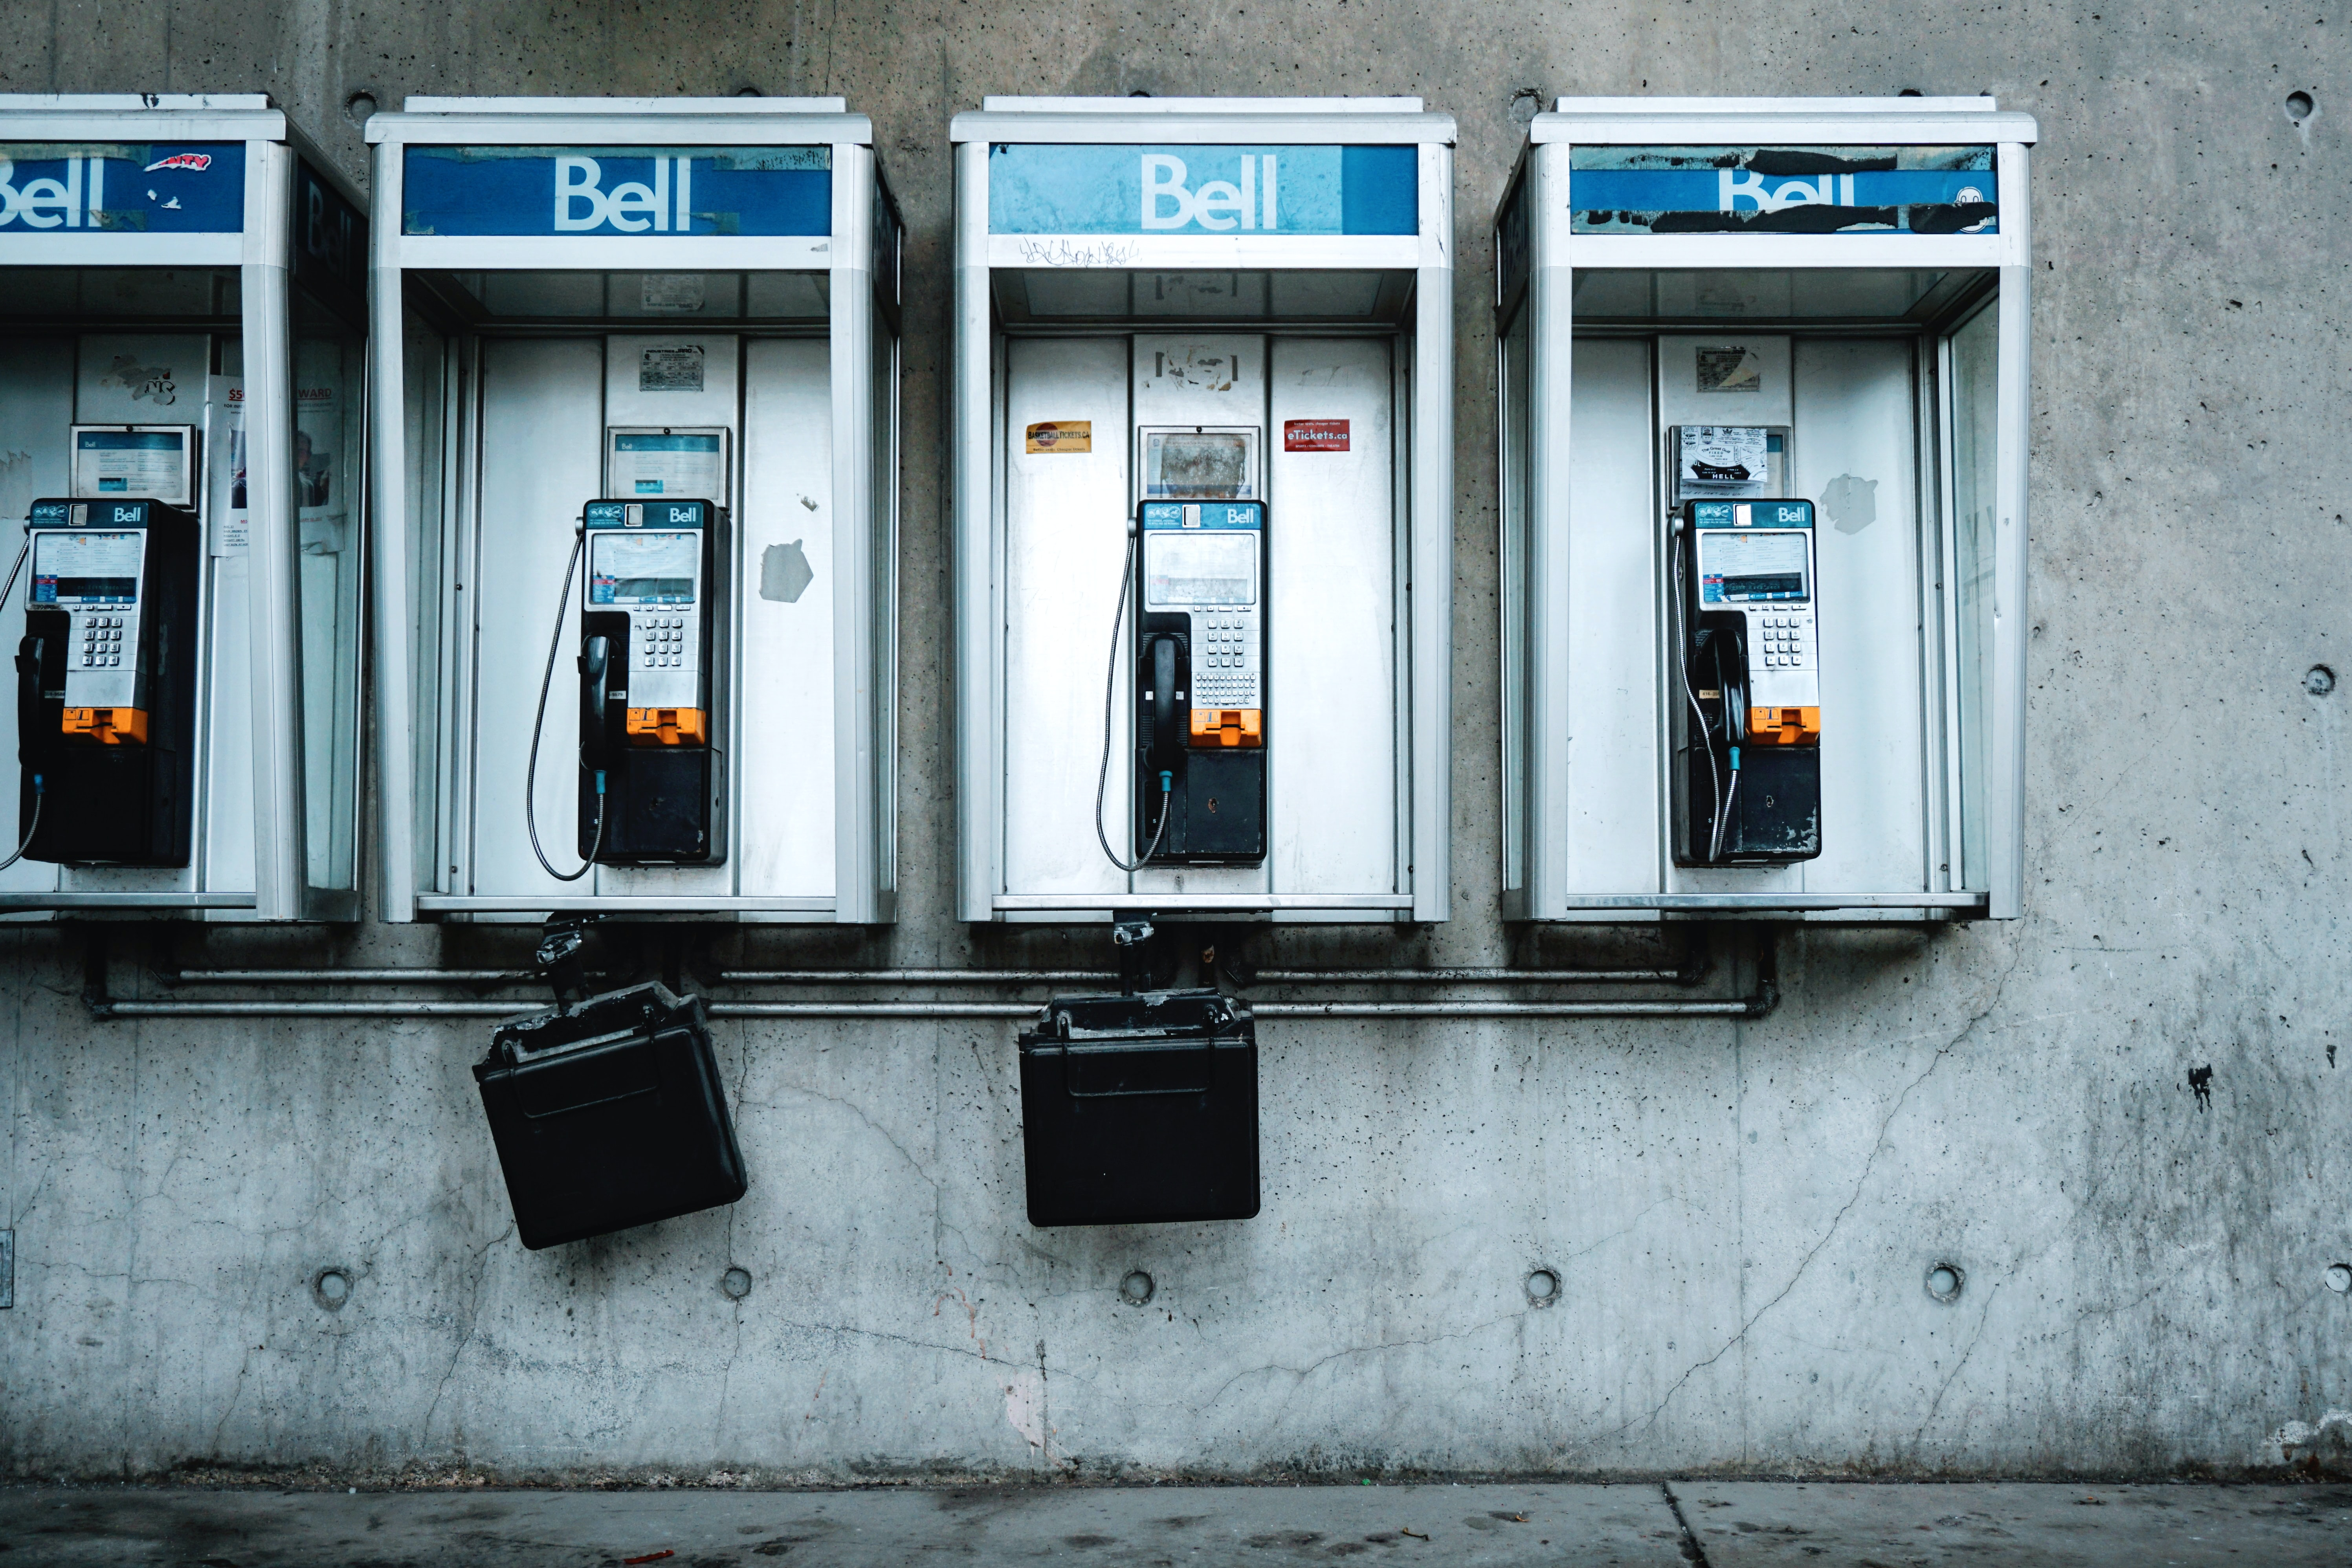
\includegraphics[width=\linewidth]{telephones.jpg}
        \end{multicols}
\end{frame}
%--- Next Frame ---%
\begin{frame}[c]{Why dynamic gossip?}
    \begin{figure}
      \begin{subfigure}[t]{.3\paperwidth}
        \centering
        
\includegraphics[height=.3\paperheight]{bitcoin.png}
        \caption*{Blockchain \cite{baird_swirlds_2016,van_renesse_blockchain_2016}}
      \end{subfigure}
      \qquad
      \begin{subfigure}[t]{.3\paperwidth}
        \centering
        
\includegraphics[height=.3\paperheight]{ssbc.png}
        \caption*{Social Media \cite{tarr_secure_2019}}
      \end{subfigure}

      \bigskip

      \begin{subfigure}[t]{.3\paperwidth}
        \centering
        
\includegraphics[height=.3\paperheight]{dna.png}
        \caption*{Genome analysis \cite{liben-nowell_gossip_2002}}
      \end{subfigure}
      \qquad
      \begin{subfigure}[t]{.3\paperwidth}
        \centering
        
\includegraphics[height=.3\paperheight]{network.pdf}
        \caption*{Distributed databases \cite{das_swim_2002,decandia_dynamo_2007}}
      \end{subfigure}
    \end{figure}
\end{frame}
%--- Next Frame ---%
\begin{frame}[c]{Some notation}
    \centering\Large
    \begin{tabular}{ll}
         Agents          & $A = \{ a, b, \dots \}$\\\pause
         Number relation & $N \subseteq A \times A$\\\pause
         Secret relation & $S \subseteq A \times A$\\\pause
         Gossip graph    & $G = (A, N, S)$\\\pause
         Call            & $ab$\\\pause
         Identity relation & $I_A = \{\ (x, x) \mid x \in A\ \}$\\
    \end{tabular}
    \vfill
\end{frame}
%--- Next Frame ---%
\begin{frame}[c]{Example}
    \centering
    \vspace{1cm}
    
    \resizebox {.7\textwidth} {!} {
        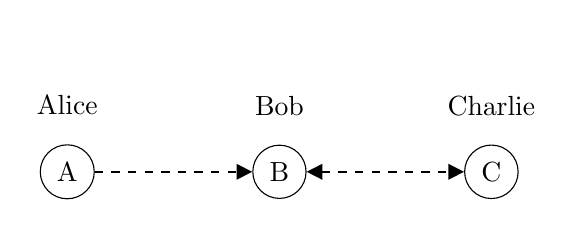
\begin{tikzpicture}[node distance=2cm]
            \node [draw, circle] (A) {A};
            \node [draw, circle, right=of A] (B) {B};
            \node [draw, circle, right=of B] (C) {C};
        
            \node [above=.25cm of A] (AName) {Alice};
            \node [above=.25cm of B] (BName) {Bob};
            \node [above=.25cm of C] (CName) {Charlie};
            
            % white text to keep spacing the same
            \node [above=1cm of B, text=white] (BName) {After call none};
        
            \draw [dashed, thick, -{Triangle[length=2mm]}] 
                (A) -- (B);
            \draw [dashed, thick, {Triangle[length=2mm]}-{Triangle[length=2mm]}] 
                (B) -- (C);
        \end{tikzpicture}
    }
    \begin{align*}
        N &= \{ (a, b), (b, c), (c, b) \} \\
        S &= I_A
    \end{align*}
\end{frame}
%--- Next Frame ---% 
\begin{frame}[c]{Example}
    \centering
    \vspace{1cm}
    
    \resizebox {.7\textwidth} {!} {
        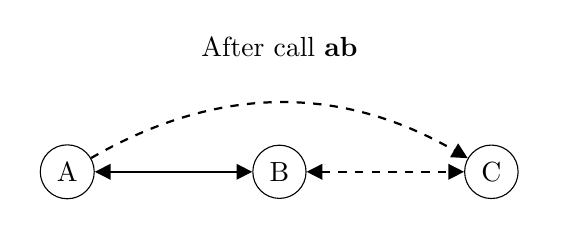
\begin{tikzpicture}[node distance=2cm]
            \node [draw, circle] (A) {A};
            \node [draw, circle, right=of A] (B) {B};
            \node [draw, circle, right=of B] (C) {C};
        
            % white text to keep spacing the same
            \node [above=.25cm of A, text=white] (AName) {Alice};
            \node [above=.25cm of B, text=white] (BName) {Bob};
            \node [above=.25cm of C, text=white] (CName) {Charlie};
            
            \node [above=1cm of B] (BName) {After call \textbf{ab}};
        
            \draw [solid, thick, {Triangle[length=2mm]}-{Triangle[length=2mm]}] 
                (A) -- (B);
            \draw [dashed, thick, -{Triangle[length=2mm]}] 
                (A) to[bend left] (C);
            \draw [dashed, thick, {Triangle[length=2mm]}-{Triangle[length=2mm]}] 
                (B) -- (C);

        \end{tikzpicture}
    }
    \begin{align*}
        N &= I_A \cup \{ (a, b), (a, c), (b, a), (b, c), (c, b) \} \\
        S &= I_A \cup \{ (a, b), (b, a) \}
    \end{align*}
\end{frame}
%--- Next Frame ---%
\begin{frame}[c]{Example}
    \centering
    \vspace{1cm}
    
    \resizebox {.7\textwidth} {!} {
        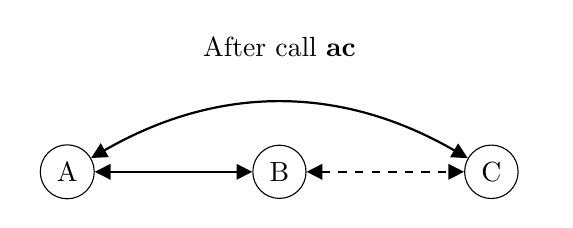
\begin{tikzpicture}[node distance=2cm]
            \node [draw, circle] (A) {A};
            \node [draw, circle, right=of A] (B) {B};
            \node [draw, circle, right=of B] (C) {C};
    
            % white text to keep spacing the same
            \node [above=.25cm of A, text=white] (AName) {Alice};
            \node [above=.25cm of B, text=white] (BName) {Bob};
            \node [above=.25cm of C, text=white] (CName) {Charlie};
            
            \node [above=1cm of B] (BName) {After call \textbf{ac}};
        
            \draw [solid, thick, {Triangle[length=2mm]}-{Triangle[length=2mm]}] 
                (A) -- (B);
            \draw [solid, thick, {Triangle[length=2mm]}-{Triangle[length=2mm]}] 
                (A) to[bend left] (C);
            \draw [dashed, thick, {Triangle[length=2mm]}-{Triangle[length=2mm]}] 
                (B) -- (C);

        \end{tikzpicture}
    }
    \begin{align*}
        N &= A \times A \\
        S &= I_A \cup \{ (a, b), (a, c), (b, a), (c, a)\}
    \end{align*}
\end{frame}
%--- Next Frame ---%
\begin{frame}[c]{Example}
    \centering
    \vspace{1cm}

    \resizebox {.7\textwidth} {!} {
        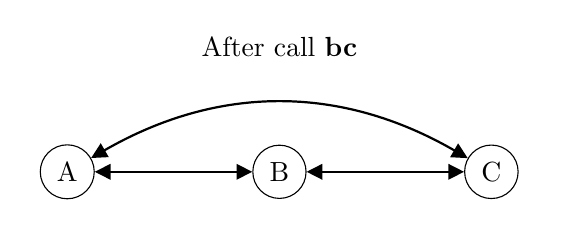
\begin{tikzpicture}[node distance=2cm]
            \node [draw, circle] (A) {A};
            \node [draw, circle, right=of A] (B) {B};
            \node [draw, circle, right=of B] (C) {C};
    
            % white text to keep spacing the same
            \node [above=.25cm of A, text=white] (AName) {Alice};
            \node [above=.25cm of B, text=white] (BName) {Bob};
            \node [above=.25cm of C, text=white] (CName) {Charlie};
            
            \node [above=1cm of B] (BName) {After call \textbf{bc}};
        
            \draw [solid, thick, {Triangle[length=2mm]}-{Triangle[length=2mm]}] 
                (A) -- (B);
            \draw [solid, thick, {Triangle[length=2mm]}-{Triangle[length=2mm]}] 
                (A) to[bend left] (C);
            \draw [solid, thick, {Triangle[length=2mm]}-{Triangle[length=2mm]}] 
                (B) -- (C);

        \end{tikzpicture}
    }
    \begin{align*}
        N &= A \times A \\
        S &= A \times A
    \end{align*}
\end{frame}
%--- Next Frame ---%
\begin{frame}[t]{The tool}
    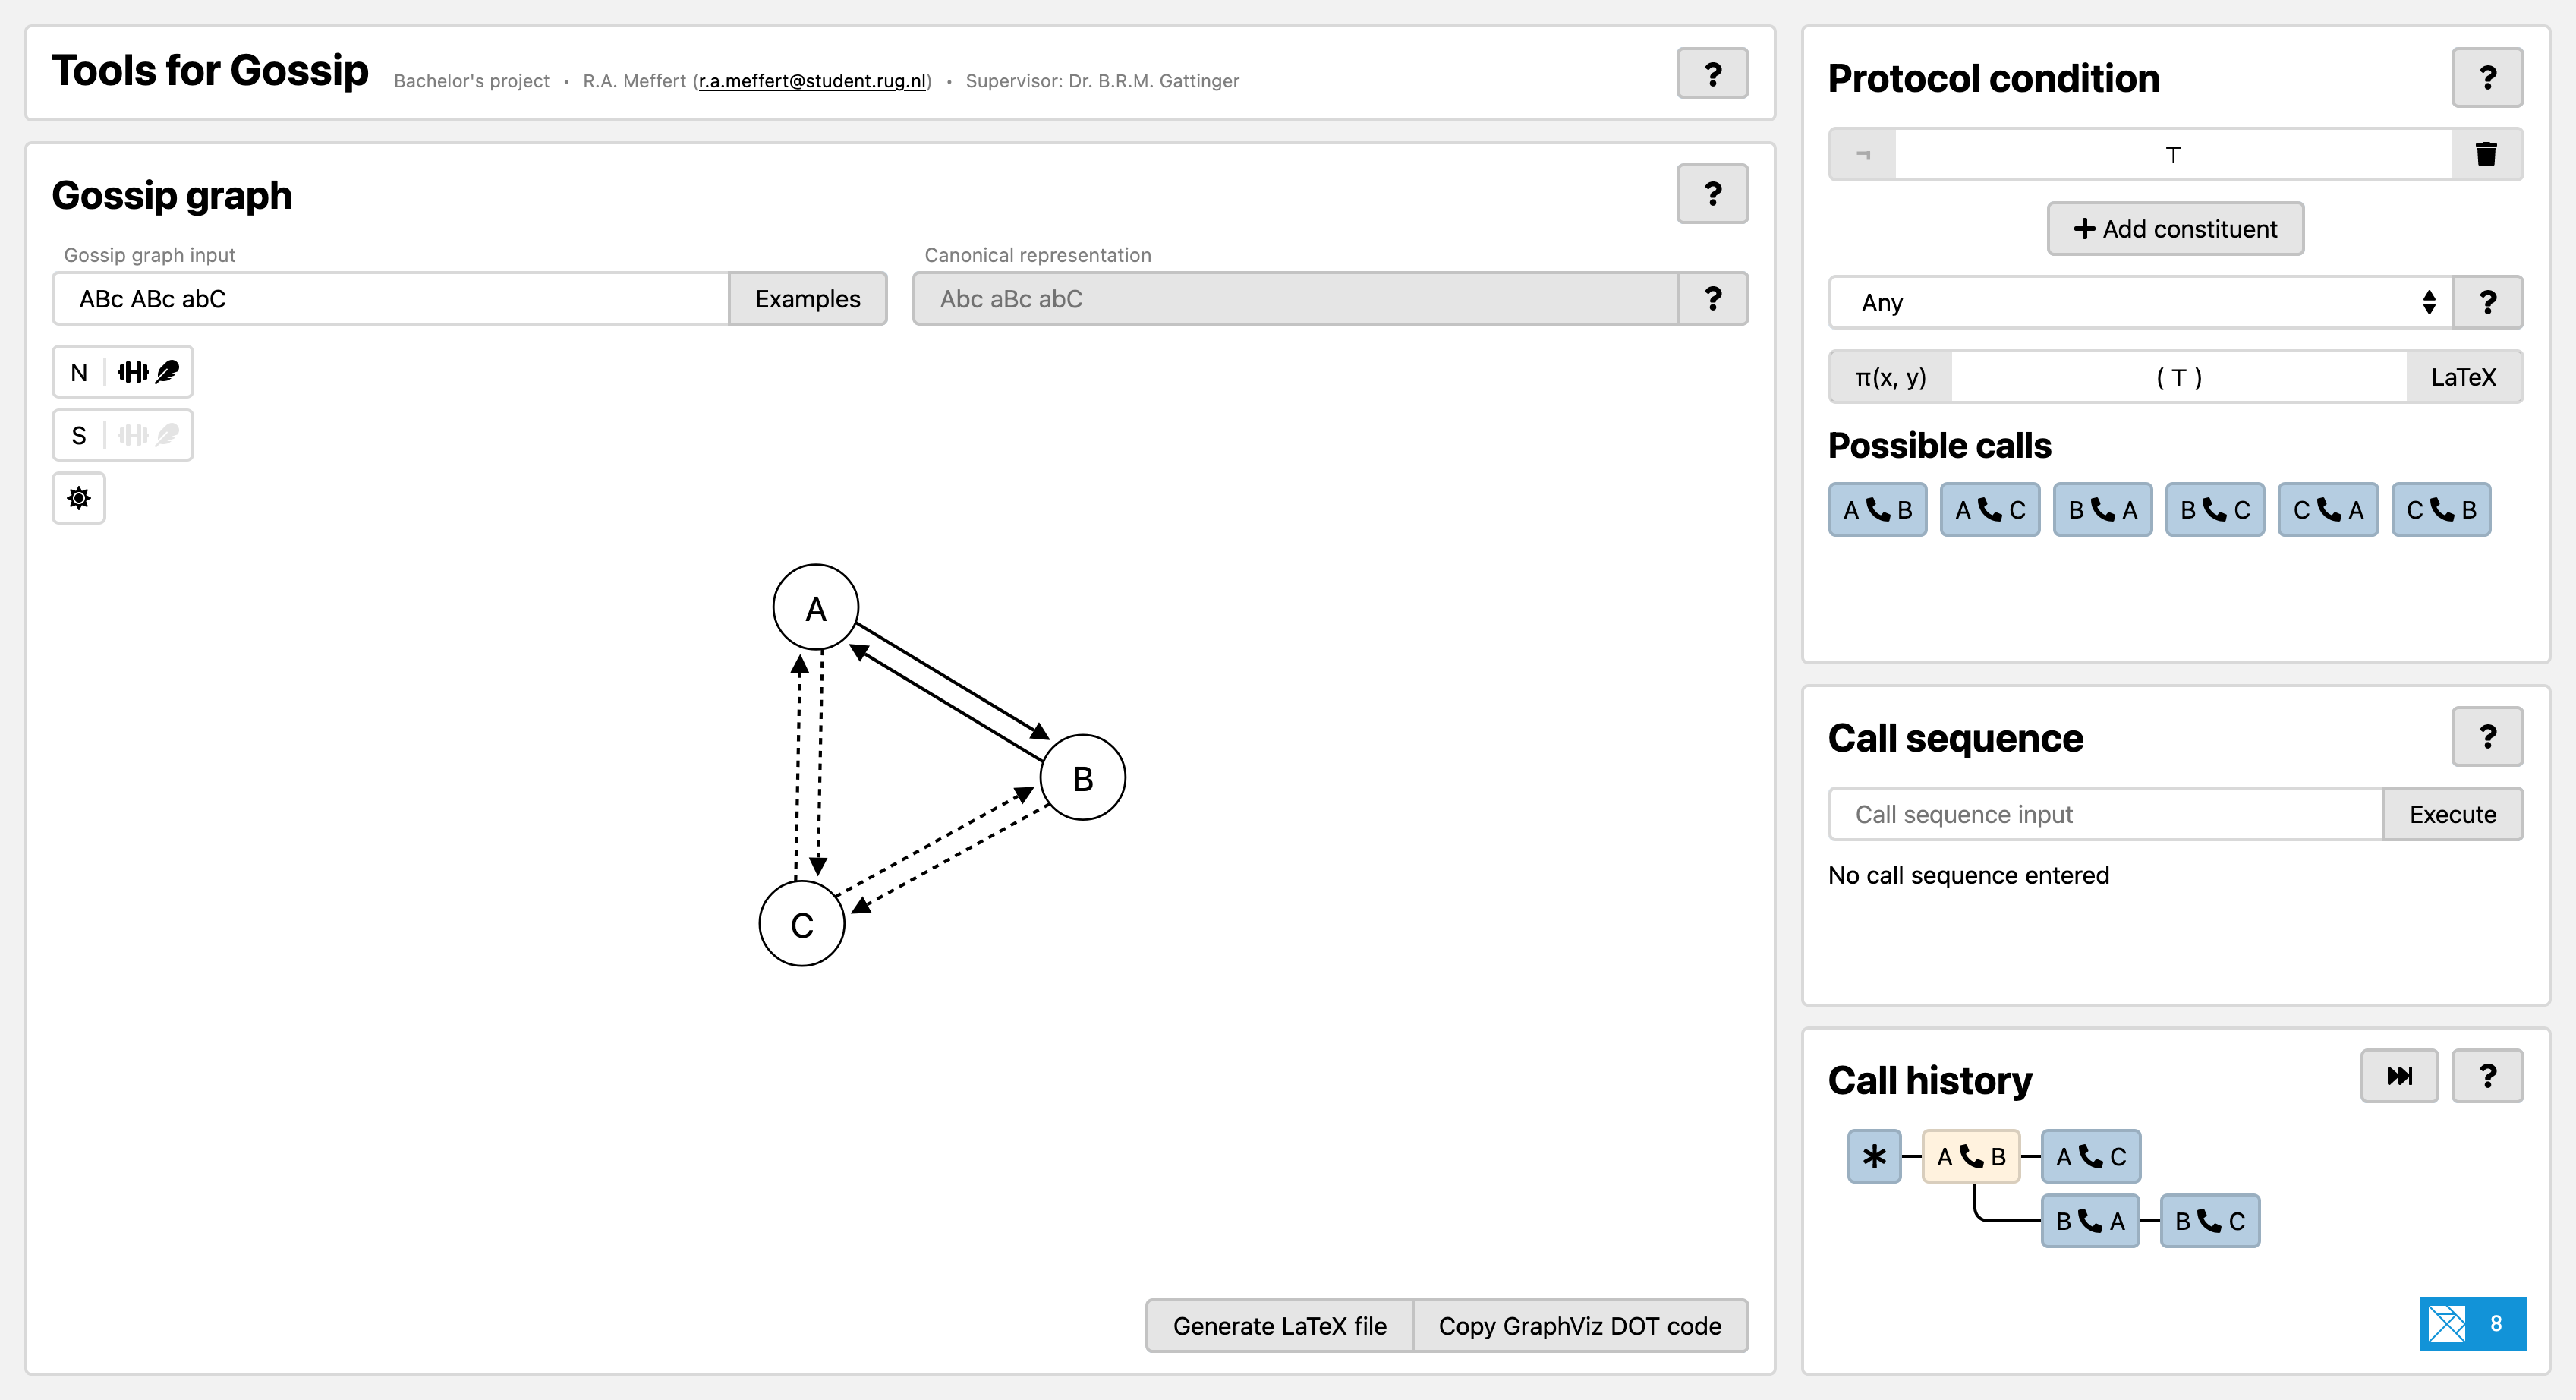
\includegraphics[width=\linewidth]{tool.png}
\end{frame}
%--- Next Frame ---%
\begin{frame}[c]{Implementation}
    \begin{multicols}{2}
        \begin{itemize}
            \item<1-> Language: Elm \cite{czaplicki_asynchronous_2013}
            \item<2-> Graph visualisation \& properties
            \item<3-> Execution tree
            \item<4-> Call sequence validation \& execution
            \item<5-> Custom protocol creation\only<5->\footnote{In last phase of development}
        \end{itemize}
        \columnbreak
        \begin{figure}
            \centering
            
\includegraphics[width=.5\linewidth]{Elm_logo.pdf}
        \end{figure}
    \end{multicols}
\end{frame}
%--- Next Frame ---%
\begin{frame}[c]{Why Elm fits this project}
    \begin{multicols}{2}
        \begin{itemize}
            \item<1-> Pure functions
            \begin{itemize}
                \item Easier to translate mathematical functions into code
            \end{itemize}
            \item<2-> Compiled to Javascript
            \begin{itemize}
                \item Free cross-platform compatibility
            \end{itemize}
            \item<3-> Static type checking
            \begin{itemize}
                \item Zero runtime exceptions
            \end{itemize}
        \end{itemize}
        \columnbreak
        \begin{figure}
            \centering
            
\includegraphics[width=.5\linewidth]{Elm_logo.pdf}
        \end{figure}
    \end{multicols}
\end{frame}
%--- Next Frame ---%
\begin{frame}[c]{Survey}
    \begin{multicols}{2}
        \begin{itemize}
            \item<1-> Short exploratory survey
            \item<2-> 12 respondents
            \item<3-> General impression: positive
            \item<4-> Useful feedback
        \end{itemize}
        \columnbreak
        \begin{figure}
            \centering
            
\includegraphics[width=\linewidth]{survey.jpg}
        \end{figure}
    \end{multicols}
\end{frame}
%--- Next Frame ---%
\begin{frame}[c]{Survey}
    \begin{figure}
        \centering
        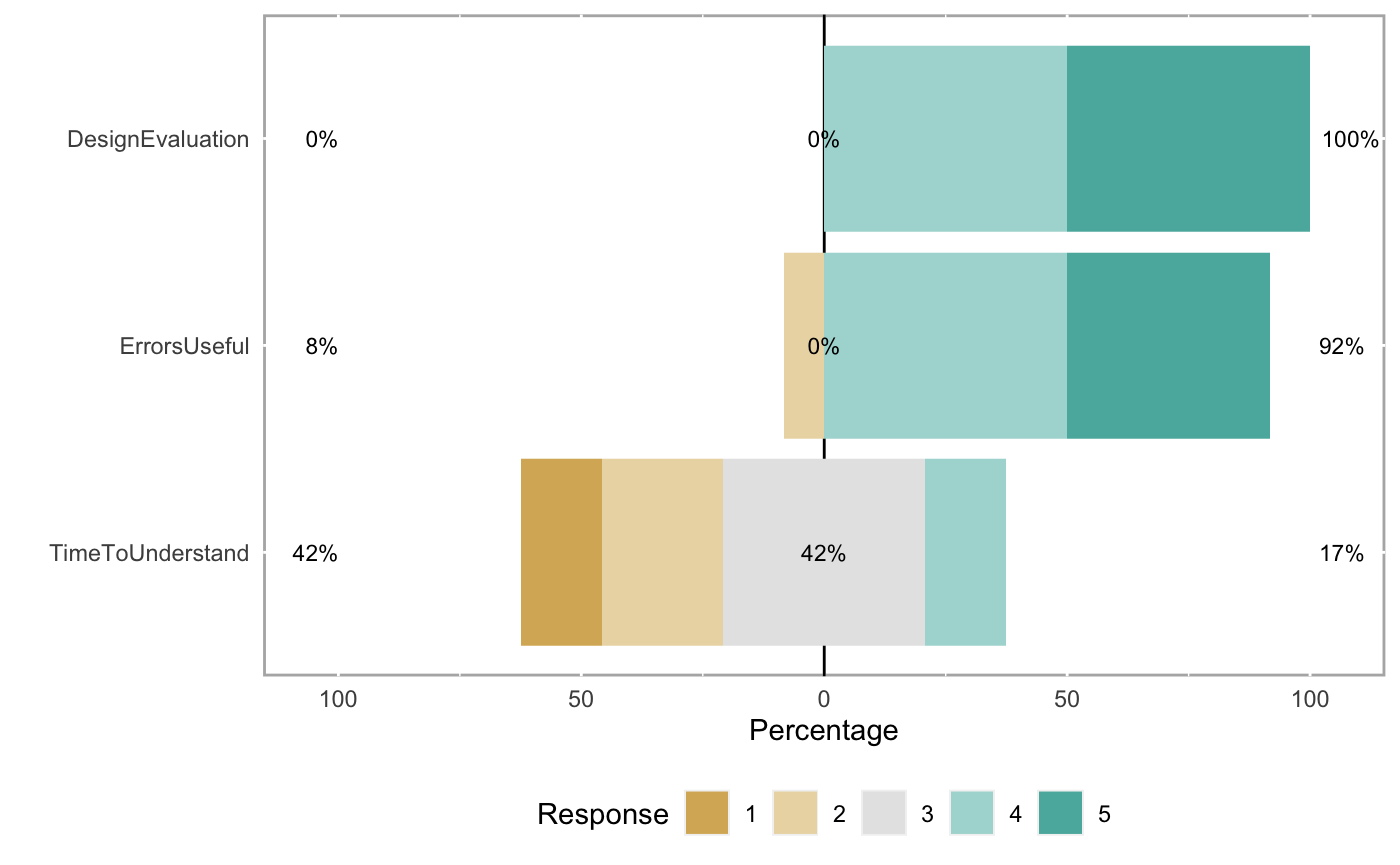
\includegraphics[width=.7\linewidth]{results.png}
        \caption*{
            \scriptsize Some results from the survey. First question was (1 = very bad) to (5 = very good), second 
            question was (1 = not useful at all) to (5 = very useful), last question was (1 = very little time) to 
            (5 = very much time). For more results, please refer to the thesis.
        }
    \end{figure}
\end{frame}
%--- Next Frame ---%
\begin{frame}[c]{Further research and extensions}
    \begin{multicols}{2}
        \begin{itemize}
            \item<1-> Unreliable gossip \cite{martins_dealing_2020}
            \item<2-> Higher level knowledge \cite{herzig_how_2017}
            \item<3-> Temporal gossip \cite{slavkovik_temporal_2019}
            \item<4-> And more!
        \end{itemize}
        \columnbreak
        \begin{figure}
            \centering
            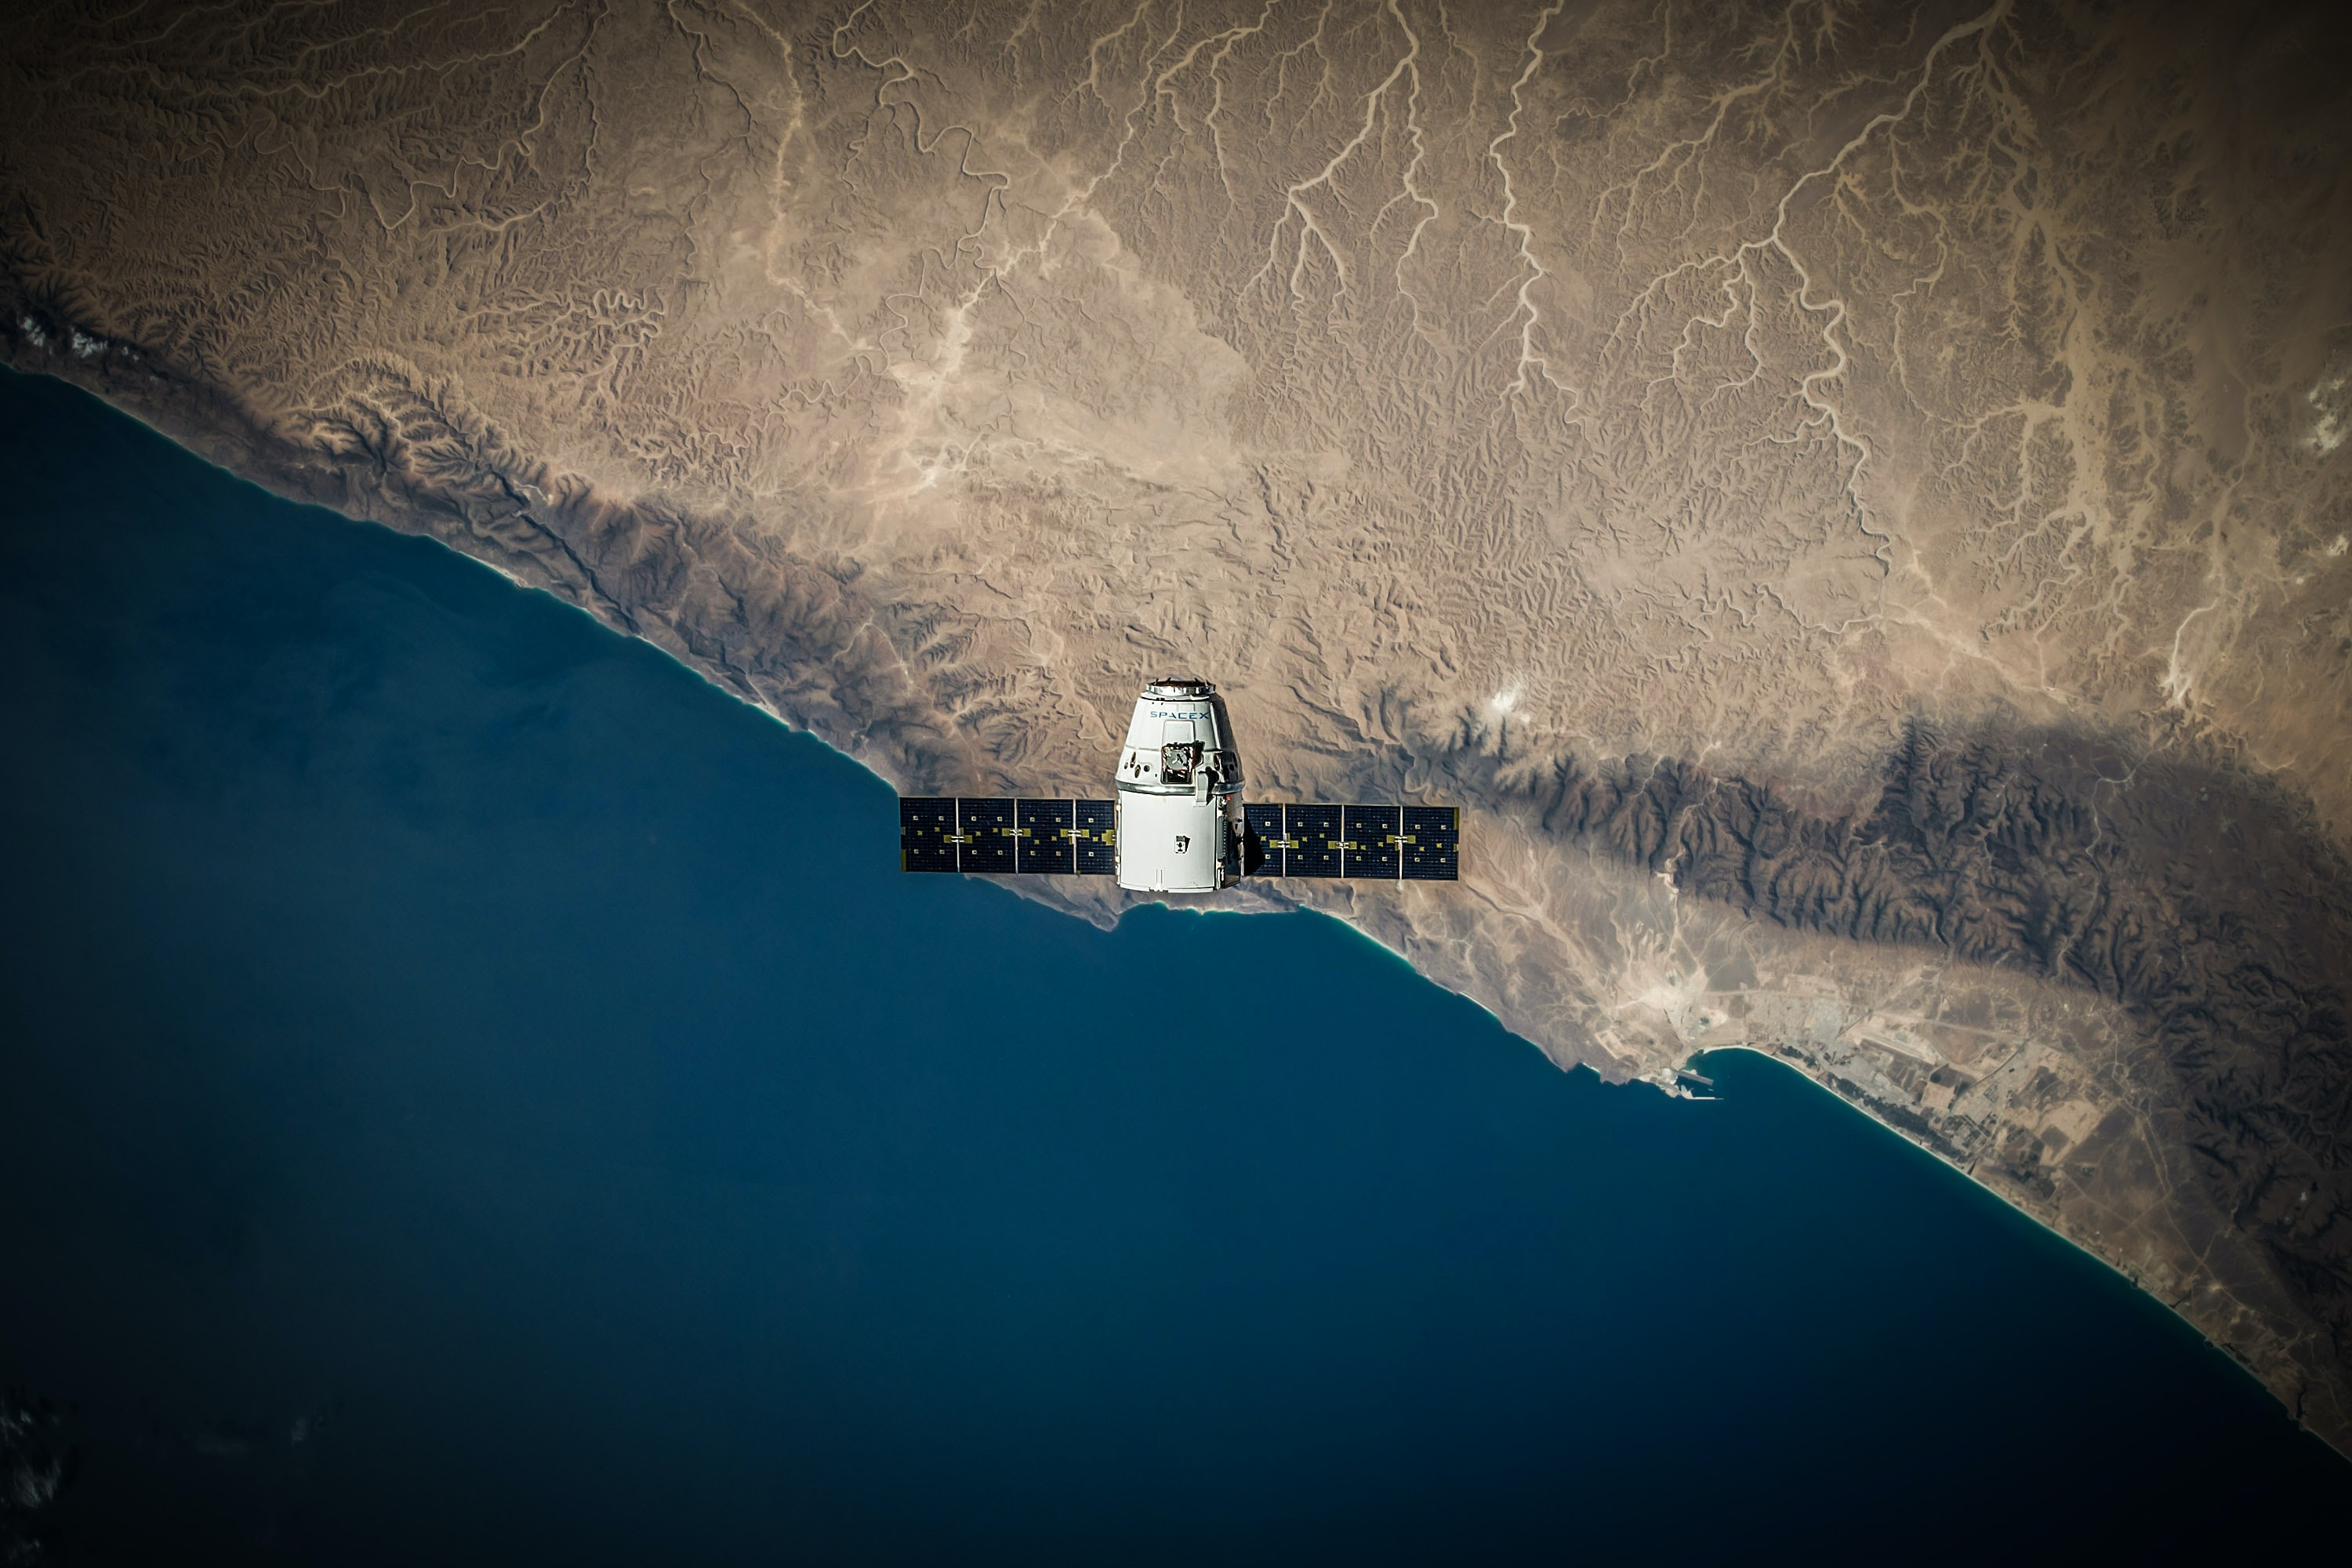
\includegraphics[width=\linewidth]{sattelite.jpg}
        \end{figure}
    \end{multicols}
\end{frame}
%--- Next Frame ---%
\begin{frame}[t]
    \Huge
    \vfill
    \vfill
    \begin{center}
        Demo
    \end{center}
    \vfill
\end{frame}
%--- Next Frame ---%
\begin{frame}[b]
    \begin{center}
        {\Large Thanks for your attention!}
        
        \bigskip
        
        Questions?
        
        \bigskip        
        \bigskip
        
        \small
        \begin{tabular}{lll}
                & Result 
                & Source code \vspace{5pt}\\
            Tool    
                & \href{https://r3n.nl/bsc/gossip}{\textcolor{gray}{r3n.nl/bsc}/gossip}
                & \href{https://r3n.nl/bsc/src/gossip}{\textcolor{gray}{r3n.nl/bsc/src}/gossip} \vspace{5pt}\\
            Thesis\footnote{From February 1}  
                & \href{https://r3n.nl/bsc/thesis}{\textcolor{gray}{r3n.nl/bsc}/thesis} 
                & \href{https://r3n.nl/bsc/src/thesis}{\textcolor{gray}{r3n.nl/bsc/src}/thesis} \vspace{5pt}\\
            Slides  
                & \href{https://r3n.nl/bsc/slides}{\textcolor{gray}{r3n.nl/bsc}/slides} 
                & \href{https://r3n.nl/bsc/src/slides}{\textcolor{gray}{r3n.nl/bsc/src}/slides} \\
        \end{tabular}
        
        \bigskip
    \end{center}
\end{frame}
%--- Next Frame ---%
\begin{frame}[t,allowframebreaks]
    \frametitle{References}
    \printbibliography
\end{frame}

\end{document}
